\documentclass[a4paper, 12pt]{report}
\usepackage[utf8]{inputenc}    
\usepackage[T1]{fontenc}
\usepackage[french]{babel}
\usepackage{hyperref}
\usepackage{setspace}
\usepackage{newtxtext,newtxmath}
\usepackage[top=3cm, bottom=3cm, left=3cm, right=3cm]{geometry}
\usepackage[explicit]{titlesec}
\usepackage{graphicx}
\usepackage[stable]{footmisc}
\usepackage{wrapfig}
\usepackage{multicol}
\usepackage{minitoc}
\usepackage{plantuml}
\usepackage{listings}

\titleformat{\chapter}[display]{}{}{0pt} {
  \parbox{\textwidth} {
    \textbf{\fontsize{30}{30}\selectfont\thechapter.\hspace{0.5cm}\LARGE#1}\\
    \rule{\textwidth}{0.4pt}
  }
}
\titleformat{name=\chapter,numberless}[display]{}{}{0pt} {
  \parbox{\textwidth}{
    \LARGE\textbf{#1}\\
    \rule{\textwidth}{0.4pt}
  }
}

\hypersetup{
    colorlinks=true,
    urlcolor=black,
    linkcolor= black,
    citecolor=black
}

\mtcsetrules{*}{off}

\onehalfspacing

\definecolor{backcolor}{rgb}{0.95,0.95,0.95}
\definecolor{numbers}{rgb}{0.5,0.5,0.5}
\lstdefinestyle{mystyle}{
    backgroundcolor=\color{backcolor},   
    aboveskip=3mm,
    belowskip=3mm,
    showstringspaces=false,
    columns=flexible,
    basicstyle={\small\ttfamily},
    numbers=none,
    breaklines=true,
    breakatwhitespace=true,
    tabsize=3,
    framexleftmargin=16pt,
    framextopmargin=6pt,
    framexbottommargin=6pt, 
    frame=tb, 
    framerule=0pt,
    numbers=left,
    numbersep=20pt,
    numberstyle=\tiny\color{numbers},
}
\lstset{style=mystyle}

\begin{document}
\renewcommand \partname{\thispagestyle{empty}}
\doparttoc

\thispagestyle{empty}
\begin{singlespace}
\begin{center}  
\begin{multicols}{2}
  \flushleft
  \null
  
\includegraphics[width=\columnwidth]{../res/logo-iut.png}
  \flushright
  \null
  \vspace{0.3cm}
  \large{Promotion 2020-2021}
\end{multicols}
\vspace{2cm}
\LARGE{\textit{Mise en place de traitements de masse relatifs à la relève des compteurs communiquants}}\\
\vspace{2cm}
\large{\textbf{Mémoire présenté en septembre 2021 par}}\\
\vspace{0.5cm}
\Large{\textit{Loïc STEINMETZ}}\\
\vspace{2cm}
\large{\textbf{En vue de l'obtention de la Licence Professionnelle}}\\
\vspace{0.5cm}
\fbox{
  \begin{minipage}{12cm}
    \begin{center}
      \null
      \vspace{0.3cm}
      \textbf{Métiers de l'Informatique}\\
      Conception, développement et test de logiciels\\
      Parcours Métiers du Génie Logiciel\\
      \null
    \end{center}
  \end{minipage}
}
\vspace{2.8cm}
\begin{multicols}{2}
  \flushleft
  \null
  \textbf{Alternance effectuée à :}\\
  Efluid\\
  2 bis, rue Ardant du Picq\\
  CS 10100 57004 METZ Cedex 01\\
  \flushright
  \null
  
\includegraphics[width=.6\columnwidth]{../res/logo-efluid.jpg}
\end{multicols}
\end{center}
\end{singlespace}

\clearpage
\thispagestyle{empty}
\null
\clearpage

\begin{singlespace}
\thispagestyle{empty}
\begin{center}  
\begin{multicols}{2}
  \flushleft
  \null
  
\includegraphics[width=\columnwidth]{../res/logo-iut.png}
  \flushright
  \null
  \vspace{0.3cm}
  \large{Promotion 2020-2021}
\end{multicols}
\vspace{2cm}
\LARGE{\textit{Mise en place de traitements de masse relatifs à la relève des compteurs communiquants}}\\
\vspace{2cm}
\large{\textbf{Mémoire présenté en septembre 2021 par}}\\
\vspace{0.5cm}
\Large{\textit{Loïc STEINMETZ}}\\
\vspace{2cm}
\large{\textbf{En vue de l'obtention de la Licence Professionnelle}}\\
\vspace{0.5cm}
\fbox{
  \begin{minipage}{12cm}
    \begin{center}
      \null
      \vspace{0.3cm}
      \textbf{Métiers de l'Informatique}\\
      Conception, développement et test de logiciels\\
      Parcours Métiers du Génie Logiciel\\
      \null
    \end{center}
  \end{minipage}
}
\vspace{2.8cm}
\begin{multicols}{2}
  \flushleft
  \null
  \textbf{Alternance effectuée à :}\\
  Efluid\\
  2 bis, rue Ardant du Picq\\
  CS 10100 57004 METZ Cedex 01\\
  \flushright
  \null
  
\includegraphics[width=.6\columnwidth]{../res/logo-efluid.jpg}
\end{multicols}
\end{center}
\end{singlespace}

\chapter*{Remerciements}
\addcontentsline{toc}{chapter}{Remerciements}
\thispagestyle{empty}

Je remercie tout particulièrement mon maître de stage, Alexandre L'Huillier, pour m'avoir fait bénéficier de ses compétences tout au long de mon année d'alternance. Merci à lui pour son professionalisme, sa confiance et sa disponibilité.

Je remercie également Jean-Luc Thiry, chef de service et Didier Grzejszczak, chef de filière, pour leur accompagnement général et pour ma bonne intégration au sein de l'entreprise.

Mes remerciements vont enfin à l'ensemble des membres du service auquel j'ai été intégré et que je n'ai pas encore cités : Patrice Frantz, Julien Kempf, Fabienne Mamet, François Molin, Roderick Pierre, Stéphane Poirot et Stéphane Roedel.

\part{Mémoire}
\renewcommand{\clearpage}{}
\chapter*{Sommaire}
\renewcommand\ptctitle{}
\parttoc
\thispagestyle{empty}
\renewcommand{\clearpage}{\newpage}
\clearpage

\chapter*{Abstract}
\addcontentsline{toc}{chapter}{Abstract}

Lorem ipsum dolor sit amet, consectetur adipiscing elit, sed do eiusmod tempor incididunt ut labore et dolore magna aliqua. Ut enim ad minim veniam, quis nostrud exercitation ullamco laboris nisi ut aliquip ex ea commodo consequat. Duis aute irure dolor in reprehenderit in voluptate velit esse cillum dolore eu fugiat nulla pariatur. Excepteur sint occaecat cupidatat non proident, sunt in culpa qui officia deserunt mollit anim id est laborum.

\chapter*{Introduction}
\addcontentsline{toc}{chapter}{Introduction}

Ce mémoire a pour objectif de présenter les travaux réalisés dans mon entreprise d'accueil, \textit{Efluid}, dans le cadre de la licence professionnelle génie logiciel, réalisée en alternance. Cette année fait suite à l'obtention de mon DUT informatique réalisée en année spéciale.

Ayant déjà réalisé mon stage de fin de DUT chez \textit{Efluid}, j'ai pu rapidement postuler à l'une des offres d'alternance que proposait le service qui m'avait déjà accueilli. Dans la continuité de mes treize semaines de stage, j'ai alors pu réintégrer ce même service pour mon année d'alternance.\\

C'est donc au sein de la division "consommation" et sous la tutelle d'Alexandre L'Huillier que j'ai pu travailler sur le projet qui m'a été confié. Je reviendrai plus loin sur la place du service dans l'organisation d'\textit{Efluid} et sur le détail du projet. On peut néanmoins résumer ainsi la formulation initiale du projet : Il s'agissait de déporter une partie des traitements réalisés en temps réel par le logiciel dans des processus lancés automatiquement et chargés de réaliser ces mêmes traitements de manière asynchrone.

Afin de mieux comprendre les enjeux et les objectifs de ce projet, je commencerai par présenter l'entreprise et son activité. Je détaillerai ensuite la nature des différentes tâches qui m'ont été confiées, ce qui me permettra de décrire le cadre de mes travaux, soit mon environnement de développement et les différents processus de production de l'entreprise. 

Il s'agira donc ensuite de détailler la mise en oeuvre du projet principal qui m'a été confié. J'expliquerai alors les différents aspects techniques et fonctionnels de mes travaux dans l'ordre de leur réalisation. Je présenterai ainsi la méthode générale mise en oeuvre et dont découle précisément cet enchaînement. 

Je concluerai enfin en présentant les différents apports de cette année d'alternance dans la perspective plus générale de mon parcours professionnel.

\chapter{Présentation de l'entreprise}

\begin{figure}[b]
  \begin{center}
    \begin{minipage}{4cm}
      \begin{center}
        
\includegraphics[height=2cm]{../res/logo-efluid.jpg}
        \caption{Efluid}
        \label{efluid}
      \end{center}
    \end{minipage}
    \rule{1cm}{0cm}
    \begin{minipage}{4cm}
      \begin{center}
        
\includegraphics[height=2cm]{../res/logo-uem.jpg}
        \caption{UEM}
        \label{uem}
      \end{center}
    \end{minipage}
    \rule{1cm}{0cm}
    \begin{minipage}{4cm}
      \begin{center}
        
\includegraphics[height=2cm]{../res/logo-enedis.jpg}
        \caption{Enedis}
        \label{enedis}
      \end{center}
    \end{minipage}
  \end{center}
\end{figure}

\section{Présentation générale}

\textit{Efluid} (\textit{cf.} figure \ref{efluid}) est une société éditrice de logiciel. Le produit qu'elle développe, portant le même nom, est un progiciel à destination des entreprises du secteur de l'énergie, qu'il s'agisse des gestionnaires de réseaux ou des distributeurs d'électricité (\textit{cf.} Annexe \ref{appendix:logiciel} : Le logiciel \textit{Efluid}). Il s'agit d'un ERP\footnote{\textit{Enterprise Resource Planning}}, ou logiciel de gestion intégré, pensé pour être adapté aux besoins spécifiques de ce secteur. Le programme est donc conçu pour pouvoir intégrer tous les aspects de cette activité, de la gestion des contrats d'énergie à la comptabilité, du chiffrage des travaux à réaliser à l'édition de documents légaux. La structure du programme est modulaire et permet donc aux clients de l'entreprise d'adapter la solution à leur besoin.\\

Cette dimension modulaire de l'application donne lieu à une division fonctionnelle des services de développement de la société, c'est-à-dire à un regrouppement des activités de développement non pas selon un critère technique (suivant par exemple l'opposition \textit{front-end}/\textit{back-end}), mais d'après les solutions apportées dans les domaines concrets de l'activité des clients (\textit{cf.} Annexe \ref{appendix:efluid-organisation} : L'organisation des services d'\textit{Efluid}). J'ai donc pour ma part été intégré à la division "consommation", qui appartient elle-même au service "comptage et réseaux". 

Outre les services de développements fonctionnels dans lesquels sont intégrés la majorité des développeurs, il existe également une filière technique dont les services sont chargés de missions transverses, comme par exemple le déploiement de l'application ou le développement des composants élémentaires du programme. C'est une partie du processus de production que j'ai moins été en mesure d'aborder au cours de mon année d'alternance, mais avec laquelle j'ai néanmoins été en contact, puisque ces services sont chargés notamment de la gestion des environnements de développement et de la maintenance des infrastructures de \textit{versionning} nécessaires aux développeurs fonctionnels.\\

\textit{Efluid} a été développé à l'initiative de l'UEM (\textit{cf.} figure \ref{uem}), en partenariat avec \textit{Enedis} (\textit{cf.} figure \ref{enedis}), qui émane d'EDF (\textit{cf.} Annexe \ref{appendix:efluid-gouvernance} : La gouvernance d'\textit{Efluid}) et profite donc de l'expertise de ces groupes afin de répondre au mieux aux besoins du secteur de l'énergie. La société est devenu un acteur important dans gestion des systèmes d'information de ce secteur et emploie aujourd'hui plus de deux-cent salariés. \textit{Efluid} compte \textit{Enedis} parmi ses clients mais aussi un grand nombre de régies locales dont par exemple l'\textit{Electricité de Strasbourg}. L'entreprise répond également a des appels d'offre à l'étranger et pourrait donc à terme prendre une dimension internationale.

\section{Spécificités du logiciel}

D'un point de vue technique, la solution applicative d'\textit{Efluid} est composée de différents modules, intégrés différement en fonction du besoin client :\\

\textit{La liste suivante est non exhaustive.}

\begin{itemize}
  \item \textit{Archi} : architecture technique
  \item \textit{Ecore} : noyau applicatif
  \item \textit{Efluid} : traitements métiers et interface web
  \item \textit{Interfaces} : gestion des échanges avec les systèmes d'information
  \item \textit{Batch} : traitements de masse exécutés de manière asynchrone
  \item \textit{Web} : gestion du serveur web
  \item \textit{Mobefluid} : application mobile
\end{itemize}
\vspace{0.5cm}

Dans le cadre des travaux qui m'ont été affectés, j'ai été amené à travailler sur les modules \textit{Ecore}, \textit{Efluid}, \textit{Interfaces} et \textit{Batch}. Conformément à mon affectation j'ai abordé principalement le domaine "consommation" au sein de ces différents modules. Il convient donc d'en mentionner les spécificités fonctionnelles.

Le traitements des consommations est une partie importance du logiciel, et consiste notamment à assurer la bonne gestion des relèves. Les relèves peuvent être de différents types, selon la nature des acteurs et des activités impliquées. En effet, une relève peut correspondre à une activité de consommation ou de production, à une mesure électrique ou gazière, être réalisée via l'intervention d'un agent, un relevé effectué par le client lui-même, ou via un compteur communiquant. Il ne s'agit là que de quelques critères parmi tous ceux qui peuvent impacter les traitements à réaliser. La gestion des relèves est donc gérée via un système complexe qui implique également de nombreux processus de calcul permettant d'intégrer les différentes grandeurs mesurées en respectant les contraintes liées à leur nature physique ainsi que les contraintes réglementaires. Il faut en outre noter que toutes ces mesures doivent pouvoir être communiquées aux différents acteurs impliqués : fournisseurs, gestionnaires de concession, clients finaux, organismes de contrôle, etc.

Ne disposant que d'une connaissance très partielle de ces différentes contraintes fonctionnelles, je ne peux pas toutes les lister ici ; une présentation détaillée de ces contraintes dépasserait en outre le cadre de ce mémoire. Cette brève description des spécificités métiers régissant le domaine consommation me permet néanmoins d'insister sur la grande complexité des traitements mis en oeuvre. On peut également noter que c'est dans la réponse à l'ensemble de ces contraintes, qu'il s'agisse de celle du domaine "consommation" ou non, que l'expertise de l'UEM a été déterminante.

Outre la grande compléxité des cas d'utilisation auxquels répond \textit{Efluid}, la solution proposée doit également répondre de certaines normes techniques négociées avec les différents clients et qui donnent lieu à des impératifs contractuels. Parmi ces spécifications techniques, on peut notamment citer les contraintes de performance auxquelles doit répondre le logiciel. Certains temps de traitement doivent par exemple correspondre à des seuils pré-déterminés, et la non-conformité des mesures de performance peut se traduire par des pénalités financières.\\

D'un point de vue général, \textit{Efluid} consiste donc en une solution applicative particulièrement complexe, ayant à répondre de nombreuses contraintes, qu'elles soient techniques ou fonctionnelles. Ce sont ces contraintes qui imposent la réalisation d'une maintenance en continu des différents traitements et l'intégration régulière de nouveaux processus. C'est précisément dans le cadre de ces contraintes générales et des contraintes propres au domaine "consommation" que s'inscrit le projet que j'ai eut à gérer. Je présenterai donc plus en profondeur certains aspects fonctionnels au moment de détailler ses objectifs.

\chapter{Sujets traités}

\section{Généralités}

Dans le cadre de mes travaux, j'ai pu appréhender l'environnement de développement propre à \textit{Efluid}, qu'il s'agisse des outils et logiciels utilisés, ou des processus de production mis en place.

\begin{figure}[b]
  \begin{center}
    \begin{minipage}{4cm}
      \begin{center}
        
\includegraphics[height=2cm]{../res/java.jpg}
        \caption{Java}
        \label{java}
      \end{center}
    \end{minipage}
    \rule{1cm}{0cm}
    \begin{minipage}{4cm}
      \begin{center}
        
\includegraphics[height=2cm]{../res/oracle.png}
        \caption{Oracle}
        \label{oracle}
      \end{center}
    \end{minipage}
    \rule{1cm}{0cm}
    \begin{minipage}{4cm}
      \begin{center}
        
\includegraphics[height=2cm]{../res/intellij.jpg}
        \vspace{0.1cm}
        \caption{Intellij}
        \label{intellij}
      \end{center}
    \end{minipage}
  \end{center}
\end{figure}

\subsection{Environnement de développement}

L'application \textit{Efluid} est développée en \textit{Java} (\textit{cf.} figure \ref{java}). C'est un langage dont j'avais déjà une certaine maîtrise avant de rejoindre l'entreprise et je n'ai donc pas eut à suivre de formation dédiée. Au delà du langage utilisé, \textit{Efluid} est  basé sur une architecture et un \textit{framework} complexe, développé initialement par CGI. La familiarisation avec la structure générale de l'application a quant à elle été plus longue et a nécessité un suivi continue durant mon année d'alternance. 

J'ai en outre bénéficié d'une formation fonctionnelle sur le logiciel, destinée aux nouveaux entrants et aux clients d'\textit{Efluid}. Cette formation portait sur des modules spécifiques de l'application, et sur l'utilisation proprement dite du logiciel. Je n'ai pour ma part suivi que la formation qui portait sur le fonctionnement du domaine "consommation" ; celle-ci m'a permis de mieux appréhender les différentes fonctionnalités du logiciel ainsi que le fonctionnement général de l'application.

Outre le \textit{Java}, j'ai aussi été amené à mobiliser mes compétence en \textit{SQL}. La base de données d'\textit{Efluid} est en effet une base \textit{Oracle} (\textit{cf.} figure \ref{oracle}) et implique donc la programmation de requêtes SQL et d'autres processus en PL/SQL, le langage propre aux bases de données \textit{Oracle}.

Les principaux logiciel que j'ai été amené à utiliser ont ainsi été \textit{Intellij} (\textit{cf.} figure \ref{intellij}) et \textit{SQL Developper}. Ce sont deux logiciels avec lesquels j'étais déjà familier et sur lesquels j'ai néanmoins été amené à approfondir mes compétences. J'ai enfin été amené à utiliser \textit{Git} comme outil de \textit{versionning}. L'intégration de \textit{Git} dans les processus de production d'\textit{Efluid} m'a permis d'appréhender une utilisation plus avancée de cet outil.

\begin{figure}[b]
  \begin{center}
    \begin{minipage}{4cm}
      \begin{center}
        \vspace{0.5cm}
        
\includegraphics[height=1cm]{../res/git.png}
        \null
        \vspace{0.5cm}
        \caption{Git}
        \label{git}
      \end{center}
    \end{minipage}
    \rule{1cm}{0cm}
    \begin{minipage}{4cm}
      \begin{center}
        
\includegraphics[height=2cm]{../res/jenkins.png}
        \caption{Jenkins}
        \label{jenkins}
      \end{center}
    \end{minipage}
    \rule{1cm}{0cm}
    \begin{minipage}{4cm}
      \begin{center}
        \vspace{0.5cm}
        
\includegraphics[height=1cm]{../res/maven.png}
        \null
        \caption{Maven}
        \label{maven}
      \end{center}
    \end{minipage}
  \end{center}
\end{figure}

\subsection{Processus de production}

Les processus de production mis en place par \textit{Efluid} reposent principalement sur quatre outils :\\

\begin{itemize}
  \item \textit{Suivefluid}
  \item \textit{Git} (\textit{cf.} figure \ref{git}), utilisé avec \textit{Gerrit}
  \item \textit{Maven} (\textit{cf.} figure \ref{maven})
  \item \textit{Jenkins} (\textit{cf.} figure \ref{jenkins})
\end{itemize}
\vspace{0.5cm}

\textit{Suivefluid} est un logiciel de suivi d'événements développé en interne et qui assure la coordination des différents services : relation client, recette et développement. Chaque développement correspond ainsi à un un événement qui se retrouve affecté à un service de développement puis à un développeur.

Suite à la réalisation du développement en question, les modifications du code sont alors synchronisées via \textit{Git}, et donnent lieu à une revue de code via \textit{Gerrit}. Une fois le développement validé, celui-ci peut alors être intégré au code source de l'application. A noter que différentes branches de développement sont gérées en même temps compte-tenu des versions en production chez les différents clients. Outre la branche de développement principale, des branches de maintenance sont en effet destinées à assurer le suivi d'anciennes versions de l'application lorsque celle-ci sont encore utilisées par certains clients.

L'ensemble des processus d'intégration et de déploiement continus sont par ailleurs administrés via \textit{Jenkins}, cet outil permettant notamment d'automatiser la compilation, les tests et le packaging de l'application. En dernière instance, ces processus sont basés sur des scripts \textit{Maven}. En effet, \textit{Maven} permet d'encapsuler l'ensemble de la configuration propre à l'application, via des fichiers POM\footnote{\textit{Project Object Model}}, qui décrivent les différentes phases du cycle de développement.\\

L'utilisation de ces outils et l'intégration plus générale des processus de production d'\textit{Efluid} m'ont permis d'appréhender les méthodes de gestion d'un projet complexe, qu'il s'agisse de son administration générale ou de la mise en place de processus de test ou de contrôle qualité. C'est donc dans ce cadre que j'ai du réaliser mes différents travaux.

\section{Développements courants}

En parallèle de mon projet principal, sur lequel je reviendrai, j'ai été amené à traiter certains événements courants. Les événements donnant lieu à un développement sont répartis chaque semaine entre les différents développeurs du service et les travaux peuvent concerner de nombreux aspects de l'application : \\

\begin{itemize}
  \item IHM \footnote{Interface Homme Machine}
  \item Traitements et algorithmes
  \item Gestion des données
  \item Gestion des logs
  \item Gestion du \textit{routing} et de la navigation
  \item \textit{Refactoring} du code existant
  \item Ecriture ou adaptation de tests
  \item Etc...
\end{itemize}
\vspace{0.5cm}

Certains projets plus longs nécessitent de passer par des procédures plus complexes, impliquant notamment les services d'analyse. La mise en oeuvre de tels projet peut alors impliquer un découpage technique : plusieurs événements peuvent correspondre à un même projet et être réparti entre plusieurs développeurs.\\

J'ai pour ma part eut à traiter notamment des corrections d'anomalies, des nouveaux développements mineurs et des travaux de \textit{refactoring}. J'ai en effet du corriger certaines anomalies au niveau de l'interface de l'application, ce qui m'a permis de mieux appréhender l'architecture générale de l'application. J'ai également du intégrer de nouveaux attributs à certains objets métiers, ce qui m'a cette fois permis d'approfondir la logique de gestion des données. J'ai enfin eut à gérer des événements de \textit{refactoring} qui m'ont permis quant à eux de mieux comprendre certains processus et traitements du logiciel, et d'approfondir ma compréhension des tests unitaires et des tests d'intégration.

D'une manière générale, la gestion de ces événements m'a permis de me familiariser progressivement avec le \textit{framework} d'\textit{Efluid}. A travers ces différents travaux j'ai en effet été amené à approfondir les différentes couches de l'architecture du logiciel, ce qui s'est avéré être très utile au moment d'aborder mon projet. C'est également à travers la gestion de ces événements que j'ai pu me familiariser avec l'ensemble des processus mis en place ainsi qu'avec les conventions et la démarche qualité propres à \textit{Efluid}. La revue de code systématique à laquelle donnent lieu les développements m'a en outre fait gagner en compétence d'un point de vue technique. J'ai en effet pu bénéficier de l'expertise des différents relecteurs concernant la logique générale de mes développements, l'utilisation de certains patrons de conception et le respect des bonnes pratiques de développement.

\section{Projet principal}

Comme indiqué en introduction, le projet principal qui m'a été attribué consistait à déporter une partie des traitements réalisés en temps réel par le logiciel dans un \textit{process} asynchrone. En d'autres termes, mon projet consistait à pouvoir gérer ces traitements en mode \textit{batch}, au lieu de les intégrer aux processus réalisés "au fil de l'eau". Dans la suite de ma présentation j'utiliserai de manière indistincte la terminologie suivante :\\

\begin{itemize}
  \item "Traitement \textit{batch}", "traitement asynchrone" : Processus automatisé, portant sur un ensemble souvent massif de données marquées spécifiquement pour donner lieu à certains traitements.
  \item "Traitement au fil de l'eau", "traitement synchrone" : Traitement réalisé en temps réel suite à une action utilisateur et portant donc uniquement sur les informations d'un contexte applicatif spécifique.
\end{itemize}
\vspace{0.5cm}

De nombreux \textit{batchs} sont intégrés à la solution applicative d'\textit{Efluid}. Comme indiqué dans la présentation générale du logiciel, les mesures de performance de l'application donnent lieu à des impératifs contractuels. Le recours à des traitements \textit{batchs} permet donc d'alléger les opérations réalisées de manière synchrone et donc d'écourter les temps de chargement lors du parcours utilisateur. Le gain de performances constituait ainsi le principal objectif de mon projet, et ce concernant un traitement en particulier correspondant à la demande de publication de la relève.

D'un point de vue fonctionnel, la demande de publication consiste à déterminer, à partir d'une relève, si les mesures enregistrées doivent être communiquées à des acteurs externes selon des critères prédéfinis, et, le cas échéant, à associer à la relève un objet portant les informations de publication. A noter que la publication proprement dite, à savoir la transmission effective des données aux acteurs concernés, est réalisée par un \textit{batch} dédié ; le périmètre de la demande de publication s'arrête quant à lui au marquage des relèves qui nécessitent une publication. Dans la situation initiale, la demande de publication était donc gérée intégralement au fil de l'eau, ce qui entrainait des temps de traitements trop longs, pouvant excéder les objectifs de performance. L'implémentation d'un \textit{batch} dédié à la demande de publication avait donc pour objectif d'alléger ces temps de traitement.\\

L'autre objectif de mon projet consistait à simplifier l'appel de la demande de publication de la relève. En l'état, la demande de publication est en effet appelée au cours de différents processus dispersés dans le code de l'application. Les traitements sont donc répétés et peuvent donner lieu à des implémentations différentes selon les contextes. Outre le gain de performance, mon projet avait donc également pour but d'implémenter un point d'accès unique à la demande de publication.

J'expliquerai plus loin pourquoi cet objectif a finalement été partiellement abandonné. Il a en effet était jugé préférable de se concentrer d'abord sur le gain de performance potentiel pouvant être réalisé.\\

Le projet tel qu'il m'a été confié était encore en phase d'analyse. En amont des travaux d'implémentation, il a donc donné lieu à une longue phase d'analyse. Une fois cette analyse réalisée, la conception technique de la solution et l'implémentation des nouveaux traitements ont été réalisés en parallèle. Je présenterai donc le traitement de mon projet industriel de manière chronologique.

\chapter{Traitement du projet industriel}

\section{Analyses préliminaires}

Lorem ipsum dolor sit amet, consectetur adipiscing elit, sed do eiusmod tempor incididunt ut labore et dolore magna aliqua. Ut enim ad minim veniam, quis nostrud exercitation ullamco laboris nisi ut aliquip ex ea commodo consequat. Duis aute irure dolor in reprehenderit in voluptate velit esse cillum dolore eu fugiat nulla pariatur. Excepteur sint occaecat cupidatat non proident, sunt in culpa qui officia deserunt mollit anim id est laborum.

\subsection{Analyse volumétrique}

Lorem ipsum dolor sit amet, consectetur adipiscing elit, sed do eiusmod tempor incididunt ut labore et dolore magna aliqua. Ut enim ad minim veniam, quis nostrud exercitation ullamco laboris nisi ut aliquip ex ea commodo consequat. Duis aute irure dolor in reprehenderit in voluptate velit esse cillum dolore eu fugiat nulla pariatur. Excepteur sint occaecat cupidatat non proident, sunt in culpa qui officia deserunt mollit anim id est laborum.

\subsection{Analyse des contextes de demande de publication de la relève}

Lorem ipsum dolor sit amet, consectetur adipiscing elit, sed do eiusmod tempor incididunt ut labore et dolore magna aliqua. Ut enim ad minim veniam, quis nostrud exercitation ullamco laboris nisi ut aliquip ex ea commodo consequat. Duis aute irure dolor in reprehenderit in voluptate velit esse cillum dolore eu fugiat nulla pariatur. Excepteur sint occaecat cupidatat non proident, sunt in culpa qui officia deserunt mollit anim id est laborum.

\subsection{Formation \textit{batch}}

Lorem ipsum dolor sit amet, consectetur adipiscing elit, sed do eiusmod tempor incididunt ut labore et dolore magna aliqua. Ut enim ad minim veniam, quis nostrud exercitation ullamco laboris nisi ut aliquip ex ea commodo consequat. Duis aute irure dolor in reprehenderit in voluptate velit esse cillum dolore eu fugiat nulla pariatur. Excepteur sint occaecat cupidatat non proident, sunt in culpa qui officia deserunt mollit anim id est laborum.

\subsection{Formalisation du périmètre fonctionnel du projet}

Lorem ipsum dolor sit amet, consectetur adipiscing elit, sed do eiusmod tempor incididunt ut labore et dolore magna aliqua. Ut enim ad minim veniam, quis nostrud exercitation ullamco laboris nisi ut aliquip ex ea commodo consequat. Duis aute irure dolor in reprehenderit in voluptate velit esse cillum dolore eu fugiat nulla pariatur. Excepteur sint occaecat cupidatat non proident, sunt in culpa qui officia deserunt mollit anim id est laborum.

\begin{figure}[b]
  \begin{center}
    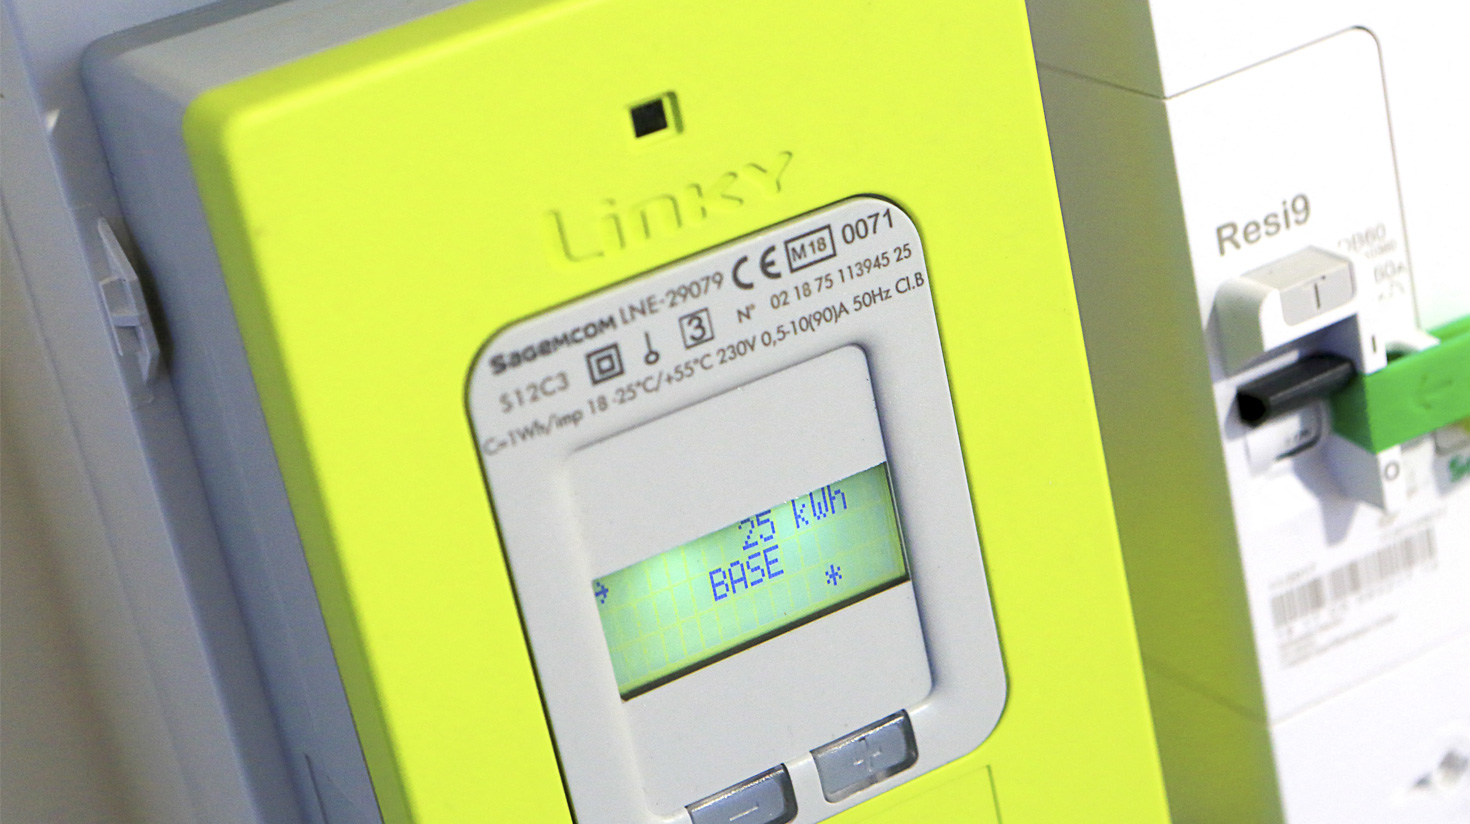
\includegraphics[height=4cm]{../res/linky.jpg}
    \caption{Compteur \textit{Linky}}
  \end{center}
\end{figure}

\section{Formalisation du besoin et planification}

Lorem ipsum dolor sit amet, consectetur adipiscing elit, sed do eiusmod tempor incididunt ut labore et dolore magna aliqua. Ut enim ad minim veniam, quis nostrud exercitation ullamco laboris nisi ut aliquip ex ea commodo consequat. Duis aute irure dolor in reprehenderit in voluptate velit esse cillum dolore eu fugiat nulla pariatur. Excepteur sint occaecat cupidatat non proident, sunt in culpa qui officia deserunt mollit anim id est laborum.

\subsection{Description fonctionnelle du \textit{batch}}

Lorem ipsum dolor sit amet, consectetur adipiscing elit, sed do eiusmod tempor incididunt ut labore et dolore magna aliqua. Ut enim ad minim veniam, quis nostrud exercitation ullamco laboris nisi ut aliquip ex ea commodo consequat. Duis aute irure dolor in reprehenderit in voluptate velit esse cillum dolore eu fugiat nulla pariatur. Excepteur sint occaecat cupidatat non proident, sunt in culpa qui officia deserunt mollit anim id est laborum.

\subsection{Découpage technique}

Lorem ipsum dolor sit amet, consectetur adipiscing elit, sed do eiusmod tempor incididunt ut labore et dolore magna aliqua. Ut enim ad minim veniam, quis nostrud exercitation ullamco laboris nisi ut aliquip ex ea commodo consequat. Duis aute irure dolor in reprehenderit in voluptate velit esse cillum dolore eu fugiat nulla pariatur. Excepteur sint occaecat cupidatat non proident, sunt in culpa qui officia deserunt mollit anim id est laborum.

\section{Conception et implémentation}

Lorem ipsum dolor sit amet, consectetur adipiscing elit, sed do eiusmod tempor incididunt ut labore et dolore magna aliqua. Ut enim ad minim veniam, quis nostrud exercitation ullamco laboris nisi ut aliquip ex ea commodo consequat. Duis aute irure dolor in reprehenderit in voluptate velit esse cillum dolore eu fugiat nulla pariatur. Excepteur sint occaecat cupidatat non proident, sunt in culpa qui officia deserunt mollit anim id est laborum.

\subsection{Solutions d'intégration du \textit{batch}}

Lorem ipsum dolor sit amet, consectetur adipiscing elit, sed do eiusmod tempor incididunt ut labore et dolore magna aliqua. Ut enim ad minim veniam, quis nostrud exercitation ullamco laboris nisi ut aliquip ex ea commodo consequat. Duis aute irure dolor in reprehenderit in voluptate velit esse cillum dolore eu fugiat nulla pariatur. Excepteur sint occaecat cupidatat non proident, sunt in culpa qui officia deserunt mollit anim id est laborum.

\subsection{Architecture générale}

Lorem ipsum dolor sit amet, consectetur adipiscing elit, sed do eiusmod tempor incididunt ut labore et dolore magna aliqua. Ut enim ad minim veniam, quis nostrud exercitation ullamco laboris nisi ut aliquip ex ea commodo consequat. Duis aute irure dolor in reprehenderit in voluptate velit esse cillum dolore eu fugiat nulla pariatur. Excepteur sint occaecat cupidatat non proident, sunt in culpa qui officia deserunt mollit anim id est laborum.

\subsection{Chargement des objets métiers}

Lorem ipsum dolor sit amet, consectetur adipiscing elit, sed do eiusmod tempor incididunt ut labore et dolore magna aliqua. Ut enim ad minim veniam, quis nostrud exercitation ullamco laboris nisi ut aliquip ex ea commodo consequat. Duis aute irure dolor in reprehenderit in voluptate velit esse cillum dolore eu fugiat nulla pariatur. Excepteur sint occaecat cupidatat non proident, sunt in culpa qui officia deserunt mollit anim id est laborum.

\subsection{Implémentation des traitements}

Lorem ipsum dolor sit amet, consectetur adipiscing elit, sed do eiusmod tempor incididunt ut labore et dolore magna aliqua. Ut enim ad minim veniam, quis nostrud exercitation ullamco laboris nisi ut aliquip ex ea commodo consequat. Duis aute irure dolor in reprehenderit in voluptate velit esse cillum dolore eu fugiat nulla pariatur. Excepteur sint occaecat cupidatat non proident, sunt in culpa qui officia deserunt mollit anim id est laborum.

\subsection{Tests}

Lorem ipsum dolor sit amet, consectetur adipiscing elit, sed do eiusmod tempor incididunt ut labore et dolore magna aliqua. Ut enim ad minim veniam, quis nostrud exercitation ullamco laboris nisi ut aliquip ex ea commodo consequat. Duis aute irure dolor in reprehenderit in voluptate velit esse cillum dolore eu fugiat nulla pariatur. Excepteur sint occaecat cupidatat non proident, sunt in culpa qui officia deserunt mollit anim id est laborum.

\chapter*{Conclusion}
\addcontentsline{toc}{chapter}{Conclusion}

Lorem ipsum dolor sit amet, consectetur adipiscing elit, sed do eiusmod tempor incididunt ut labore et dolore magna aliqua. Ut enim ad minim veniam, quis nostrud exercitation ullamco laboris nisi ut aliquip ex ea commodo consequat. Duis aute irure dolor in reprehenderit in voluptate velit esse cillum dolore eu fugiat nulla pariatur. Excepteur sint occaecat cupidatat non proident, sunt in culpa qui officia deserunt mollit anim id est laborum.

\part{Annexes}
\renewcommand{\clearpage}{}
\chapter*{Table des annexes}
\renewcommand\ptctitle{}
\parttoc
\thispagestyle{empty}
\renewcommand{\clearpage}{\newpage}
\appendix

\chapter{\textit{Efluid} : logiciel}
\label{appendix:logiciel}

\begin{center}
  
\includegraphics[height=7.5cm]{../res/efluid-1.png}
  \null
  \vspace{0.3cm}
  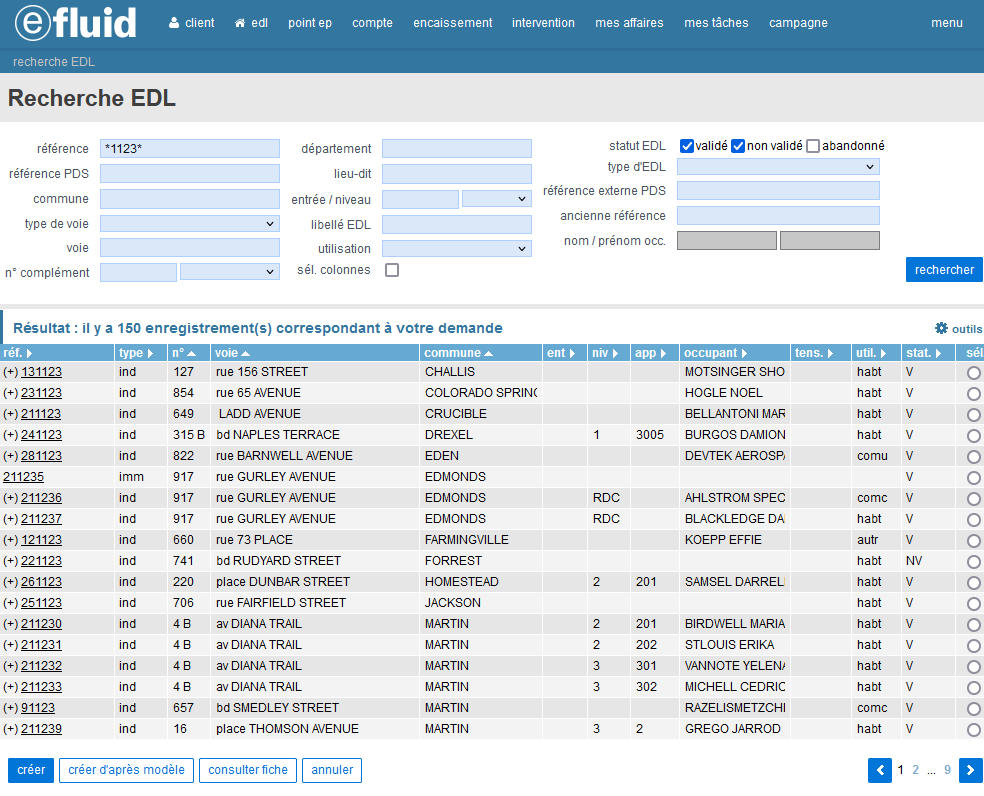
\includegraphics[height=9cm]{../res/efluid-2.png}
\end{center}

\chapter{\textit{Efluid} : organisation des services}
\label{appendix:efluid-organisation}

\begin{center}
  \begin{plantuml}
    @startmindmap
    
    <style>
      node {
          LineColor black
          BackgroundColor #FFF
          RoundCorner 0
      }
      arrow {
          LineColor #000
      }
      grey {
        BackgroundColor #BBB
      }
    </style>

      * Direction générale
      ** Direction informatique
      *** Technologies
      *** Développement : CRM et Facturation
      *** Développement : Comptage et réseaux <<grey>>
      ** Direction commerciale
      *** Expertise fonctionnelle : CRM et Facturation
      *** Expertise fonctionnelle : Comptage et réseaux
      *** Coordination et clients
      *** Prestation et projets
      ** Ginko

    @endmindmap
  \end{plantuml}
\end{center}

\vspace{1cm}
\noindent\textbf{CRM :} \textit{Customer Relationship Management}, gestion de la relation client.\\
\noindent\textbf{Ginko :} Système d'information d'\textit{Enedis} lié aux compteurs communiquants.

\chapter{\textit{Efluid} : gouvernance}
\label{appendix:efluid-gouvernance}

\begin{center}
  \begin{plantuml}
    @startmindmap
    
    <style>
      node {
          LineColor black
          BackgroundColor #FFF
          RoundCorner 0
      }
      arrow {
          LineColor #000
      }
      grey {
        BackgroundColor #BBB
      }
    </style>

      * Efluid
      **_ 60%
      *** UEM
      **_ 30%
      *** Enedis
      **_ 10%
      *** CDC

    @endmindmap
  \end{plantuml}
\end{center}

\vspace{1cm}
\noindent\textbf{UEM :} Usine d'Electricité de Metz.\\
\noindent\textbf{CDC :} Caisse des Dépôts et Consignations.

\chapter{Volumétrie}
\label{appendix:volumetrie}

\textit{Volumes estimés le 20/01/2021 à partir des copies anonymisées des bases de données de production.}\\

Les données suivantes permettent d’évaluer le nombre de relèves concernées par le processus de demande de publication quel que soit leur contexte de création.\\

\begin{itemize}
  \item \textbf{UEM}
  \begin{itemize}
    \item \approx\space 3 500 relèves impliquant une création d'échange
    \item \approx\space 91 000 relèves créées
    \item Ratio demande de publication / création de relève : \approx\space 4\%
  \end{itemize}
  \item \textbf{Enedis IDF}
  \begin{itemize}
    \item \approx\space 6 300 000 relèves impliquant une création d'échange
    \item \approx\space 6 400 000 relèves créées
    \item Ratio demande de publication / création de relève : \approx\space 99\%
  \end{itemize}
  \item \textbf{Enedis Est}
  \begin{itemize}
    \item \approx\space 3 000 000 relèves impliquant une création d'échange
    \item \approx\space 3 100 000 relèves créées
    \item Ratio demande de publication / création de relève : \approx\space 95\%
  \end{itemize}
  \item \textbf{Enedis Ouest}
  \begin{itemize}
    \item \approx\space 5 200 000 relèves impliquant une création d'échange
    \item \approx\space 5 400 000 relèves créées
    \item Ratio demande de publication / création de relève : \approx\space 96\%
  \end{itemize}
  \item \textbf{Enedis Méditerranée}
  \begin{itemize}
    \item \approx\space 5 200 000 relèves impliquant une création d'échange
    \item \approx\space 5 400 000 relèves créées
    \item Ratio demande de publication / création de relève : \approx\space 96\%
  \end{itemize}
\end{itemize}
\clearpage

Les données suivantes permettent d’évaluer le nombre de relèves concernées par le processus de demande de publication en ne considérant que les relèves réalisées via un compteur \textit{\textit{Linky}}.\\

\begin{itemize}
  \item \textbf{Enedis IDF}
  \begin{itemize}
    \item \approx\space 5 400 000 relèves de compteurs \textit{\textit{Linky}} impliquant une création d'échange
    \item \approx\space 5 500 000 relèves de compteur \textit{\textit{Linky}} créées
    \item Ratio demande de publication / création de relève : \approx\space 98\%
    \item \approx\space 85\% des relèves créées concernent un compteur \textit{\textit{Linky}}
    \item \approx\space 85\% des demandes de publication de la relève concernent une relève de compteur \textit{\textit{Linky}}
  \end{itemize}
  \item \textbf{Enedis Est}
  \begin{itemize}
    \item \approx\space 2 500 000 relèves de compteurs \textit{Linky} impliquant une création d'échange
    \item \approx\space 2 600 000 relèves de compteur \textit{Linky} créées
    \item Ratio demande de publication / création de relève : \approx\space 95\%
    \item \approx\space 89\% des relèves créées concernent un compteur \textit{Linky}
    \item \approx\space 85\% des demandes de publication de la relève concernent une relève de compteur \textit{Linky}
  \end{itemize}
  \item \textbf{Enedis Ouest}
  \begin{itemize}
    \item \approx\space 4 600 000 relèves de compteurs \textit{Linky} impliquant une création d'échange
    \item \approx\space 4 800 000 relèves de compteur \textit{Linky} créées
    \item Ratio demande de publication / création de relève : \approx\space 96\%
    \item \approx\space 89\% des relèves créées concernent un compteur \textit{Linky}
    \item \approx\space 90\% des demandes de publication de la relève concernent une relève de compteur \textit{Linky}
  \end{itemize}
  \item \textbf{Enedis Méditerranée}
  \begin{itemize}
    \item \approx\space 4 800 000 relèves de compteurs \textit{Linky} impliquant une création d'échange
    \item \approx\space 4 900 000 relèves de compteur \textit{Linky} créées
    \item Ratio demande de publication / création de relève : \approx\space 97\%
    \item \approx\space 90\% des relèves créées concernent un compteur \textit{Linky}
    \item \approx\space 91\% des demandes de publication de la relève concernent une relève de compteur \textit{Linky}
  \end{itemize}
\end{itemize}

\chapter{Planification}
\label{appendix:planification}

\begin{itemize}
  \item \textbf{Planification annuelle :}\\
\end{itemize}

\begin{center}
  \begin{plantuml}
    @startuml

    skinparam monochrome true
    scale 1024 width
    scale 768 height

    printscale monthly zoom 1.4
    project starts the 2020-09-01

    [Pré-conception] starts 2020-09-01
    [Pré-conception] ends 2020-12-31
    [Conception] starts 2020-12-01
    [Conception] ends 2021-05-31
    [Développements] starts 2021-03-01
    [Développements] ends 2021-08-31

    @enduml
  \end{plantuml}
\end{center}
\vspace{1cm}

\begin{itemize}
  \item \textbf{Planification de l'implémentation :}\\
\end{itemize}

\begin{center}
  \begin{plantuml}
    @startuml

    skinparam monochrome true
    scale 1024 width
    scale 768 height

    printscale weekly
    project starts the 2021-02-01

    [Formalisation du besoin] starts 2021-02-01
    [Formalisation du besoin] ends 2021-02-15
    --
    [Intégration de la solution] starts 2021-02-08
    [Intégration de la solution] ends 2021-03-07
    --
    [Squelette batch] starts 2021-03-01
    [Squelette batch] ends 2021-03-15
    --
    [Implémentation des chargements] starts 2021-03-16
    [Implémentation des chargements] ends 2021-05-01
    --
    [Implémentation des process] starts 2021-04-16
    [Implémentation des process] ends 2021-06-01
    --
    [Tests] starts 2021-06-01
    [Tests] ends 2021-07-31

    [Squelette batch]->[Implémentation des chargements]
    [Implémentation des chargements]->[Tests]
    [Implémentation des process]->[Tests]
    [Intégration de la solution]->[Tests]

    @enduml
  \end{plantuml}
\end{center}

\chapter{Traitement de la demande de publication}
\label{appendix:process}

\begin{itemize}
  \item \textbf{Structure des traitements :}\\
\end{itemize}

\begin{center}
  \begin{plantuml}
    @startuml

    skinparam monochrome true
    left to right direction

    GestionDemandePublicationReleveProcess <|-- GestionDemandePublicationAvecDonneesProcess
    GestionDemandePublicationReleveProcess <|-- GestionDemandePublicationEstimationReleveFacturationProcess
    GestionDemandePublicationReleveProcess <|-- GestionDemandePublicationImportReleveAvecDonneesProcess

    @enduml
  \end{plantuml}
\end{center}
\vspace{0.5cm}

\begin{itemize}
  \item \textbf{Processus appelants :}\\
  \begin{itemize}
    \item Saisie d'une relève par un agent
    \item Auto-relève lors d'une demande de prestation
    \item CRI\footnote{Compte-Rendu d'Intervention} avec saisie d'une relève
    \item REL005MT : \textit{Batch} de calcul des consommations
    \item REL019MT : \textit{Batch} d'import des télérelèves gaz
    \item FAC002MT : \textit{Batch} d'estimation des relèves pour EDP\footnote{Elément De Population} facturable
    \item FAC006MT : \textit{Batch} de calcul des factures
    \item FAC020MT : \textit{Batch} d'estimation des relèves pour EDP non factuable
    \item \underline{LKY06} : Interface de récupération des données \textit{Linky}
  \end{itemize}
\end{itemize}

\chapter{\textit{Design Pattern}\footnote{Patron de conception} : Stratégie}
\label{appendix:strategy}

\begin{itemize}
  \item \textbf{Sans stratégie :}\\
\end{itemize}

\begin{center}
  \begin{plantuml}
    @startuml

    skinparam monochrome true
    scale 200 height

    class Process {
      executer() : void
    }
    class SousProcess1 {
      executer1() : void
    }
    class SousProcess2 {
      executer2() : void
    }
    class SousProcess3 {
      executer3() : void
    }

    Process ..> SousProcess1
    Process ..> SousProcess2
    Process ..> SousProcess3

    @enduml
  \end{plantuml}
\end{center}
\vspace{0.5cm}

\begin{lstlisting}
public class Process {

    public void executer() {
        if (condition1) {
          new SousProcess1().exectuer1();
        } else if (condition2) {
          new SousProcess2().executer2();
        } else if (condition3) {
          new SousProcess3.executer3();
        }
    }    
}
\end{lstlisting}
\clearpage

\begin{itemize}
  \item \textbf{Avec stratégie :}\\
\end{itemize}

\begin{center}
  \begin{plantuml}
    @startuml

    skinparam monochrome true

    class Process {
      -service : Service
      +executer() : void
    }
    interface Service {
      +executerService() : void
    }
    class SousProcess1 {
      +executerService() : void
    }
    class SousProcess2 {
      +executerService() : void
    }
    class SousProcess3 {
      +executerService() : void
    }

    Process *-- Service
    Service <-- SousProcess1
    Service <-- SousProcess2
    Service <-- SousProcess3

    @enduml
  \end{plantuml}
\end{center}
\vspace{0.5cm}

\begin{lstlisting}
  public class Process {

      private Service service;

      public Process(Service service) {
        this.service = service;
      }
  
      public void executer() {
          service.executerService();
      }    
  }
  \end{lstlisting}

\chapter{\textit{Batch} : architecture et implémentation}
\label{appendix:batch}

\begin{itemize}
  \item \textbf{Architecture :}\\
\end{itemize}

\begin{center}
  \begin{plantuml}
    @startuml

    scale 450 height
    skinparam monochrome true

    abstract class ProgramBatchDAO
    abstract class ProgramBatch
    class ParallelJobLauncher
    abstract class AbstractAppBatchJob
    abstract class BatchJobDAO

    ProgramBatch .u.> ProgramBatchDAO
    ProgramBatch .d.> ParallelJobLauncher
    ParallelJobLauncher .d.> AbstractAppBatchJob
    AbstractAppBatchJob .d.> BatchJobDAO

    @enduml
  \end{plantuml}
\end{center}
\clearpage

\begin{itemize}
  \item \textbf{Implémentation :}\\
\end{itemize}

\begin{center}
  \begin{plantuml}
    @startuml

    skinparam monochrome true
    scale 250 height

    class DemandePublicationRekeveProgramDAO
    class ERequeteDemandePublicationReleveBatchDAO
    class DemandePublicationReleveJobDAO

    DemandePublicationRekeveProgramDAO .d.> ERequeteDemandePublicationReleveBatchDAO
    DemandePublicationReleveJobDAO .u.> ERequeteDemandePublicationReleveBatchDAO

    @enduml
  \end{plantuml}
\end{center}
\begin{center}
  \begin{plantuml}
    @startuml

    skinparam monochrome true
    scale 150 height

    class DemandePublicationReleveProgram
    class DemandePublicationReleveBatchConstantes

    DemandePublicationReleveProgram .d.> DemandePublicationReleveBatchConstantes

    @enduml
  \end{plantuml}
\end{center}
\begin{center}
  \begin{plantuml}
    @startuml

    skinparam monochrome true
    left to right direction

    class DemandePublicationReleveJob
    class GestionDemandePublicationReleveProcess #BBB
    class ECountDemandePublicationReleveType
    class DemandePublicationReleveBatchDAOExceptions

    DemandePublicationReleveJob ..> GestionDemandePublicationReleveProcess
    DemandePublicationReleveJob ..> ECountDemandePublicationReleveType
    DemandePublicationReleveJob ..> DemandePublicationReleveBatchDAOExceptions

    @enduml
  \end{plantuml}
\end{center}

\tableofcontents
\thispagestyle{empty}

\chapter*{Résumé}
\thispagestyle{empty}

Lorem ipsum dolor sit amet, consectetur adipiscing elit, sed do eiusmod tempor incididunt ut labore et dolore magna aliqua. Ut enim ad minim veniam, quis nostrud exercitation ullamco laboris nisi ut aliquip ex ea commodo consequat. Duis aute irure dolor in reprehenderit in voluptate velit esse cillum dolore eu fugiat nulla pariatur. Excepteur sint occaecat cupidatat non proident, sunt in culpa qui officia deserunt mollit anim id est laborum.

\end{document}